% !TEX TS-program = XeLaTeX
% use the following command: 
% all document files must be coded in UTF-8
\documentclass{textolivre}
% for anonymous submission
%\documentclass[anonymous]{textolivre}
% to create HTML use 
%\documentclass{textolivre-html}
% See more information on the repository: https://github.com/leolca/textolivre

% Metadata
\begin{filecontents*}[overwrite]{article.xmpdata}
    \Title{O socioconstrutivismo, a literacia e o trabalho com TICs durante a pandemia de Coronavírus em 2020}
    \Author{Janete Rosa da Fonseca \sep Lovania Roehrig Teixeira \sep David Arenas Carmona}
    \Language{pt-BR}
    \Keywords{Literacia \sep Ensino remoto \sep Socioconstrutivismo}
    \Journaltitle{Texto Livre}
    \Journalnumber{1983-3652}
    \Volume{14}
    \Issue{2}
    \Firstpage{1}
    \Lastpage{9}
    \Doi{10.35699/1983-3652.2021.34333}

    \setRGBcolorprofile{sRGB_IEC61966-2-1_black_scaled.icc}
            {sRGB_IEC61966-2-1_black_scaled}
            {sRGB IEC61966 v2.1 with black scaling}
            {http://www.color.org}
\end{filecontents*}

% used to create dummy text for the template file
\definecolor{dark-gray}{gray}{0.35} % color used to display dummy texts
\usepackage{lipsum}
\SetLipsumParListSurrounders{\colorlet{oldcolor}{.}\color{dark-gray}}{\color{oldcolor}}

% used here only to provide the XeLaTeX and BibTeX logos
\usepackage{hologo}

% used in this example to provide source code environment
%\crefname{lstlisting}{lista}{listas}
%\Crefname{lstlisting}{Lista}{Listas}
%\usepackage{listings}
%\renewcommand\lstlistingname{Lista}
%\lstset{language=bash,
        breaklines=true,
        basicstyle=\linespread{1}\small\ttfamily,
        numbers=none,xleftmargin=0.5cm,
        frame=none,
        framexleftmargin=0.5em,
        framexrightmargin=0.5em,
        showstringspaces=false,
        upquote=true,
        commentstyle=\color{gray},
        literate=%
           {á}{{\'a}}1 {é}{{\'e}}1 {í}{{\'i}}1 {ó}{{\'o}}1 {ú}{{\'u}}1 
           {à}{{\`a}}1 {è}{{\`e}}1 {ì}{{\`i}}1 {ò}{{\`o}}1 {ù}{{\`u}}1
           {ã}{{\~a}}1 {ẽ}{{\~e}}1 {ĩ}{{\~i}}1 {õ}{{\~o}}1 {ũ}{{\~u}}1
           {â}{{\^a}}1 {ê}{{\^e}}1 {î}{{\^i}}1 {ô}{{\^o}}1 {û}{{\^u}}1
           {ä}{{\"a}}1 {ë}{{\"e}}1 {ï}{{\"i}}1 {ö}{{\"o}}1 {ü}{{\"u}}1
           {Á}{{\'A}}1 {É}{{\'E}}1 {Í}{{\'I}}1 {Ó}{{\'O}}1 {Ú}{{\'U}}1
           {À}{{\`A}}1 {È}{{\`E}}1 {Ì}{{\`I}}1 {Ò}{{\`O}}1 {Ù}{{\`U}}1
           {Ã}{{\~A}}1 {Ẽ}{{\~E}}1 {Ũ}{{\~u}}1 {Õ}{{\~O}}1 {Ũ}{{\~U}}1
           {Â}{{\^A}}1 {Ê}{{\^E}}1 {Î}{{\^I}}1 {Ô}{{\^O}}1 {Û}{{\^U}}1
           {Ä}{{\"A}}1 {Ë}{{\"E}}1 {Ï}{{\"I}}1 {Ö}{{\"O}}1 {Ü}{{\"U}}1
           {ç}{{\c{c}}}1 {Ç}{{\c{C}}}1
}


\journalname{Texto Livre}
\thevolume{14}
\thenumber{2}
\theyear{2021}
\receiveddate{\DTMdisplaydate{2020}{12}{11}{-1}} % YYYY MM DD
\accepteddate{\DTMdisplaydate{2021}{02}{28}{-1}}
\publisheddate{\DTMdisplaydate{2021}{07}{2}{-1}}
% Corresponding author
\corrauthor{Janete Rosa da Fonseca}
% DOI
\articledoi{10.35699/1983-3652.2021.34333}
% list of available sesscions in the journal: articles, dossier, reports, essays, reviews, interviews, editorial
\articlesessionname{dossier}
% Abbreviated author list for the running footer
\runningauthor{Fonseca et al.}
\editorname{Anna Izabella M. Pereira}

\title{O socioconstrutivismo, a literacia e o trabalho com TICs durante a pandemia de Coronavírus em 2020}
\othertitle{Socioconstructivism, literacy and working with ICTs during the Coronavirus pandemic in 2020}
% if there is a third language title, add here:
%\othertitle{Artikelvorlage zur Einreichung beim Texto Livre Journal}

\author[1]{Janete Rosa da Fonseca \orcid{0000-0001-7732-0385} \thanks{Email: \url{janete.fonseca@ufms.br}}}
\author[2]{Lovania Roehrig Teixeira \orcid{0000-0001-9614-8648} \thanks{Email: \url{lovania.teixeira@ufms.br}}}
\author[1]{David Arenas Carmona \orcid{0000-0002-6737-6235} \thanks{Email: \url{dav.are.car@gmail.com}}}

\affil[1]{Universidade Federal de Mato Grosso do Sul, Curso de Pedagogia - Câmpus de Aquidauana, Aquidauana, Mato Grosso do Sul, Brasil.}
\affil[2]{Universidade Federal de Mato Grosso do Sul, Curso de Letras - Câmpus de Aquidauana, Aquidauana, Mato Grosso do Sul, Brasil.}

\addbibresource{article.bib}
% use biber instead of bibtex
% $ biber tl-article-template

% set language of the article
\setdefaultlanguage{portuguese}
\setotherlanguage{english}

% for spanish, use:
%\setdefaultlanguage{spanish}
%\gappto\captionsspanish{\renewcommand{\tablename}{Tabla}} % use 'Tabla' instead of 'Cuadro'
%\AfterEndPreamble{\crefname{table}{tabla}{tablas}\Crefname{table}{Tabla}{Tablas}}

% for languages that use special fonts, you must provide the typeface that will be used
% \setotherlanguage{arabic}
% \newfontfamily\arabicfont[Script=Arabic]{Amiri}
% \newfontfamily\arabicfontsf[Script=Arabic]{Amiri}
% \newfontfamily\arabicfonttt[Script=Arabic]{Amiri}
%
% in the article, to add arabic text use: \textlang{arabic}{ ... }

% to use emoticons in your manuscript
% https://stackoverflow.com/questions/190145/how-to-insert-emoticons-in-latex/57076064
% using font Symbola, which has full support
% the font may be downloaded at:
% https://dn-works.com/ufas/
% add to preamble:
% \newfontfamily\Symbola{Symbola}
% in the text use:
% {\Symbola }

% reference itens in a descriptive list using their labels instead of numbers
% insert the code below in the preambule:
\makeatletter
\let\orgdescriptionlabel\descriptionlabel
\renewcommand*{\descriptionlabel}[1]{%
  \let\orglabel\label
  \let\label\@gobble
  \phantomsection
  \edef\@currentlabel{#1\unskip}%
  \let\label\orglabel
  \orgdescriptionlabel{#1}%
}
\makeatother
%
% in your document, use as illustraded here:
%\begin{description}
%  \item[first\label{itm1}] this is only an example;
%  % ...  add more items
%\end{description}
 

% custom epigraph - BEGIN 
%%% https://tex.stackexchange.com/questions/193178/specific-epigraph-style
\usepackage{epigraph}
\renewcommand\textflush{flushright}
\makeatletter
\newlength\epitextskip
\pretocmd{\@epitext}{\em}{}{}
\apptocmd{\@epitext}{\em}{}{}
\patchcmd{\epigraph}{\@epitext{#1}\\}{\@epitext{#1}\\[\epitextskip]}{}{}
\makeatother
\setlength\epigraphrule{0pt}
\setlength\epitextskip{0.5ex}
\setlength\epigraphwidth{.7\textwidth}
% custom epigraph - END


% if you use multirows in a table, include the multirow package
\usepackage{multirow}

% add line numbers for submission
%\usepackage{lineno}
%\linenumbers

\begin{document}
\maketitle

\begin{polyabstract}
\begin{abstract}
Este artigo busca discutir os pontos positivos e negativos do trabalho de ensino-aprendizagem da literacia \cite{morais2013, morais2014} durante a pandemia de coronavírus em 2020 de um ponto de vista de uma teoria socioconstrutivista \cite{vygotski1991}. Assim, especificamente, buscamos discutir como a utilização de diferentes Tecnologias da Informação e Comunicação (TICs) exerce influência no desenvolvimento da leitura e da escrita, na fase de alfabetização de crianças, especialmente quais os papéis e os atores desse processo e como se verifica o alcance da zona de desenvolvimento proximal (ZDP) do discente. Um dos pontos negativos do uso exclusivo de TICs no ensino, tanto em atividades síncronas como assíncronas, é a dificuldade de diagnóstico do nível de aprendizagem dos discentes. Afinal, por meio do ensino presencial, é possível acompanhar o progresso do aluno durante o processo de alfabetização e, assim, verificar o desenvolvimento da ZDP de diversas formas. Um dos pontos positivos do uso de TICs é a valorização da autonomia do discente no processo de ensino-aprendizagem de leitura e de escrita e, assim, também ocorre o reconhecimento do papel de mediador do docente. Além disso, os familiares (pais, avós, irmãos, etc.) que acompanham essa criança durante as aulas remotas também passam a atuar em certa medida, assim como os docentes, como mediadores do processo de ensino-aprendizagem.

\keywords{Literacia \sep Ensino remoto \sep Socioconstrutivismo}
\end{abstract}

\begin{english}
\begin{abstract}
This paper intends to discuss the positive and negative points of literacy teaching-learning work \cite{morais2013, morais2014} during the coronavirus pandemic in 2020 from the point of view of a socio-constructivist theory \cite{vygotski1991}. Thus, specifically, we intend to discuss how the use of different Information and Communication Technologies (ICTs) impacts on the development of reading and writing, in the children's literacy phase, especially which are the roles and actors of this process and how is verified the student's proximal development zone (PDZ). A negative point of the exclusive use of ICTs in teaching, both in synchronous and asynchronous activities, is the difficulty in diagnosing the students' level of learning. After all, through face-to-face teaching, it is possible to check the student's progress during the literacy process and, thus, diagnose the development of the PDZ by several ways. A positive point is the valorization of the student's autonomy in the teaching-learning process of reading and writing and, thus, there is also an appreciation of the teacher's mediating role. In addition, family members (parents, grandparents, etc.) who accompany this child during remote classes also start to act, as well as teachers, as mediators in the teaching-learning process.

\keywords{Literacy \sep Remote teaching \sep Socioconstructivism.}
\end{abstract}
\end{english}

% if there is another abstract, insert it here using the same scheme
\end{polyabstract}


\section{Introdução}\label{intro}
O objetivo deste artigo é discutir qual é e como se dá o impacto do uso exclusivo de TICs no ensino-aprendizagem da literacia na fase de alfabetização nos primeiros anos do Ensino Fundamental no contexto de uma emergência de saúde pública como a pandemia de COVID-19 em 2020. Especificamente, de um ponto de vista do sociocontrutivismo, buscamos levantar os pontos positivos e negativos que o uso das TICs durante a pandemia de COVID-19 suscitou. 

O ano de 2020 obrigou o Brasil e o mundo a se reinventar, o que aconteceu também no contexto educacional. Devido à impossibilidade de se ter aulas presenciais em 2020, devido ao risco de propagação do coronavírus, as escolas tiveram de desenvolver alternativas e assumir meios de desenvolver o ensino-aprendizagem que não gerassem aglomerações e, assim, se respeitasse o distanciamento físico sugerido pelos órgãos de saúde. Assim, o sistema educacional público e privado teve de se reformular e lançar mão de TICs para que alunos não “perdessem” o ano letivo. Essa solução paliativa e de emergência recebeu vários nomes tais como “ensino remoto emergencial” e “aulas on-line”. Dado esse contexto particular, neste artigo buscamos discutir, a partir do ponto de vista de uma abordagem socioconstrutivista, como o ensino-aprendizagem se desenvolveu em 2020 e como o uso das TICs dificultou ou facilitou o processo no que diz respeito aos primeiros anos do Ensino Fundamental e, especificamente, no desenvolvimento da literacia na fase de alfabetização. Para realizar isso, inicialmente, discutiremos alguns aspectos relacionados à literacia na alfabetização, em seguida, apresentaremos alguns dos principais pressupostos da teoria socioconstrutivista, depois, discutiremos os pontos positivos e negativos do ensino remoto e o uso de TICs em 2020 no que diz respeito ao desenvolvimento da literacia. Finalmente, apresentaremos as considerações finais.

\section{Alfabetização e literacia}\label{alfab}
Nesta seção abordaremos alguns aspectos importantes relacionando a alfabetização à literacia nos anos iniciais do Ensino Fundamental e alguns marcos legais importantes que tratam sobre esses temas.

Um marco na história das normativas sobre a alfabetização no Brasil foi a homologação, em 2017, da Base Nacional Comum Curricular (BNCC), um documento regulador e padronizador dos currículos das escolas públicas e privadas que propõe conteúdos mínimos para cada etapa da escolarização. “Conforme a BNCC, espera-se que a criança seja alfabetizada no 1º e 2º ano do ensino fundamental, processo que será complementado por outro, a partir do 3º ano, denominado “ortografização” \cite[p. 14]{brasil2019}.

Segundo o Programa Nacional de Alfabetização \cite{brasil2019} foi divulgado o relatório do \emph{National Reading Panel} em 2000 e nele se identificaram cinco elementos cruciais para uma alfabetização efetiva e de qualidade: a consciência fonêmica, a instrução fônica sistemática, a fluência de leitura, o vocabulário e a compreensão de textos \cite{nationalreading2000}. “Esses pilares passaram a sustentar os bons programas de alfabetização e a ser recomendados em diversos países” \cite[p. 16]{brasil2019}.

Na sequência, em 2009, o relatório \emph{Developing Early Literacy} \cite{nationalearly2009} afirmou que 

\begin{quote}
[...] quanto maior o envolvimento dos pais na etapa da educação infantil (por meio da leitura em voz alta e de conversas mais elaboradas com seus filhos, por exemplo), mais habilidades de literacia a criança poderá adquirir. O relatório tratou também das habilidades fundamentais para a alfabetização desenvolvidas na pré-escola, como o conhecimento do nome, dos sons e das formas das letras e a aquisição da consciência fonológica e fonêmica \cite[p. 16]{brasil2019}.
\end{quote}

Em vista desses relatórios e descobertas, criou-se a Política Nacional de Alfabetização (doravante, PNA) que “[...] se propõe a assumir e a difundir tais contribuições, ora aprimoradas pelas evidências científicas mais recentes. E uma das mais importantes consiste em adotar um conceito claro e objetivo de alfabetização” \cite[p. 17]{brasil2019}.

O PNA define alfabetização como o ensino das habilidades de leitura e de escrita em um sistema alfabético que representa com os caracteres do alfabeto (letras) os sons da fala \cite{morais2014}. Outro conceito importante é o de princípio alfabético. Um indivíduo ao compreendê-lo entende que “[...] os caracteres alfabéticos não são meros sinais gráficos, mas que, individualmente ou em grupo, representam os sons da fala (ou os fonemas da língua) ” \cite[p. 18]{brasil2019}. Cada língua tem suas regras específicas de correspondência grafema-fonema e assim o princípio se concretiza diferentemente em cada uma delas. Nesse contexto, a alfabetização requer um ensino explícito e sistemático, numa ordem que segue na direção do mais simples para o mais complexo \cite[p. 18]{brasil2019}. 

A alfabetização leva ao desenvolvimento da literacia. O termo “literacia”, por sua vez, refere-se ao conjunto das habilidades da leitura e da escrita (identificação das palavras escritas, conhecimento da ortografia das palavras, aplicação aos textos dos processos linguísticos e cognitivos de compreensão), isto é, é o conjunto de conhecimentos, habilidades e atitudes relacionados à leitura e à escrita, bem como sua prática produtiva \cite{morais2013, morais2014}. Desse modo, a literacia envolve o desenvolvimento amplo e efetivo da alfabetização rumo à leitura e à escrita de textos com autonomia.

Na PNA explica-se o porquê do uso do termo “literacia”:

\begin{quote}
O conceito de literacia vem se difundindo desde os anos 1980 e nas políticas públicas se reveste de especial importância como fator para o exercício pleno da cidadania. É termo usado comumente em Portugal e em outros países lusófonos, equivalente a \emph{literacy} do inglês e a \emph{littératie do francês}. A opção por utilizá-lo traz diversas vantagens, pois é uma forma de alinhar-se à terminologia científica consolidada internacionalmente \cite[p. 21]{brasil2019}.
\end{quote}

O desenvolvimento da literacia comporta 3 diferentes níveis que consistem em habilidades adquiridas antes da alfabetização e consolidadas depois dela \cite[p. 21]{brasil2019}. Na pirâmide abaixo (\Cref{fig1}) estão representados os diferentes níveis de literacia baseados no modelo de Timothy Shanahan e Cynthia Shanahan \cite{shanahan2008}.

\begin{figure}[htbp]
 \centering
 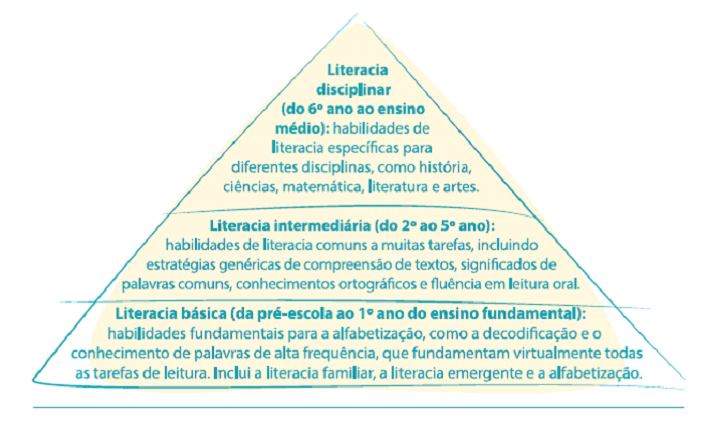
\includegraphics[width=0.75\textwidth]{fig.png}
 \caption{Níveis de Literacia}
 \label{fig1}
 \source{\cite[p. 21]{brasil2019}}
\end{figure}

Conforme \textcite[p. 43-44]{shanahan2008}, na base da pirâmide (da pré-escola ao fim do 1º ano do ensino fundamental), está a literacia básica, que inclui a aquisição das habilidades fundamentais para a alfabetização (literacia emergente), como o conhecimento de vocabulário e a consciência fonológica, bem como as habilidades adquiridas durante a alfabetização, isto é, a aquisição das habilidades de leitura (decodificação) e de escrita (codificação). No processo de aprendizagem, essas habilidades básicas devem ser consolidadas para que a criança possa acessar conhecimentos mais complexos. Além disso, 

\begin{quote}
[s]tudents also come to expect certain organizational or structural properties in texts, such as the basic problem-centered formulation of stories or the list structure in simple expository texts, and they come to assume the presence of an author, though their conception of authoris not particularly rhetorical, intentional, or separate from the reader’s own perspective \cite[p. 44]{shanahan2008}.
\end{quote}

No segundo nível, está a \textbf{literacia intermediária} (do 2º ao 5º ano do ensino fundamental), que abrange habilidades mais avançadas, como a fluência em leitura oral, que é necessária para a compreensão de textos \cite[p. 21]{brasil2019}. Além disso,  

\begin{quote}
[s]tudents also gain access to more complex forms of text organization (e.g., parallel plots, circular plots, problem-solution, cause-effect), and begin to use author intention as a general tool for critical response (that is, they start to infer author purpose and to consider the implications of the choices that emanate from such a purpose) \cite[p. 45]{shanahan2008}.
\end{quote}

No topo da pirâmide (do 6º ano ao ensino médio), está o nível de \textbf{literacia disciplinar}, onde se encontram as habilidades de leitura aplicáveis a conteúdos específicos de disciplinas, como geografia, biologia e história \cite[p. 21]{brasil2019}, o conjunto de conhecimentos, habilidades e atitudes relacionados à leitura e à
escrita, desenvolvidos antes da alfabetização pois

\begin{quote}
[...] during [...] high school, many students begin to master even more specialized reading routines and language uses, and these particular outcomes, although powerful and valuable, are also more constrained in their applicability to most reading tasks. The constraints on the generalizability of literacy skills for more advanced readers — symbolized here by the narrowing of the pyramid — are imposed by the increasingly disciplinary and technical turn in the nature of literacy tasks \cite[p. 45]{shanahan2008}.
\end{quote}

Já é consolidado na literatura \cite[entre outros]{shanahan2008, wasik2004, senechal2008} que se uma criança, antes de dar início ao processo formal da alfabetização, desenvolve atividades de literacia emergente e de literacia familiar sua alfabetização e toda sua vida escolar posterior também é favorecida. A \textbf{literacia emergente}, pode-se dizer, é o conjunto de conhecimentos, habilidades e atitudes relacionados à leitura e à escrita, desenvolvidos antes da alfabetização \cite[p. 22]{brasil2019}. Em suma, na literacia emergente incluem-se experiências e conhecimentos sobre a leitura e a escrita adquiridos de maneira lúdica e adequada à idade da criança, de modo formal ou informal, antes de aprender a ler e a escrever \cite[p. 22]{brasil2019}.

Segundo \textcite{wasik2004, senechal2008}, a \textbf{literacia familiar} também tem impacto positivo na alfabetização. O êxito das crianças na aprendizagem da leitura e da escrita está vinculado ao ambiente familiar e às práticas e experiências relacionadas à linguagem, à leitura e à escrita que elas vivenciam com seus pais, familiares ou cuidadores, mesmo antes do ingresso no ensino formal. 

Assim, a alfabetização e o restante da vida escolar da criança são influenciados pelas atividades de interação, tanto com a oralidade quanto com a escrita, desenvolvidas na família e antes da instrução formal. Em consequência disso, depois do início da alfabetização, a literacia se consolida com mais robustez e o sujeito adquire cada vez mais autonomia e capacidade de lidar com os recursos linguísticos disponíveis na língua. Nesse contexto, quanto maior e mais cedo ocorrer o envolvimento da família em atividades de literacia e, por isso, no processo de ensino-aprendizagem, mais benefícios a criança terá no momento da alfabetização e depois dela.

\section{Abordagem socioconstrutivista de Vygotsky}\label{abordagem}
Nesta seção abordaremos alguns aspectos importantes para o escopo deste artigo relacionados à teoria socioconstrutivista vygostkyana, tais como a zona de desenvolvimento proximal (doravante, ZDP) e o papel do mediador no desenvolvimento e na aprendizagem. 

A teoria socioconstrutivista se baseia na ideia de que a aprendizagem e o desenvolvimento ocorrem em um contexto social. Para \textcite{vygotski1991} “a aprendizagem da criança começa muito antes da aprendizagem escolar”. Desse modo, para o autor, a criança entra em uma escola e seu desenvolvimento ocorre (ou não) a partir do conhecimento adquirido em casa, na família, em seu bairro, etc. Assim, aprendizagem e desenvolvimento se relacionam desde o nascimento de uma criança e não somente quando ela adentra em uma instituição formal de ensino.  Logo, a criança não é um quadro em branco quando chega à escola, como o behaviorismo de \cite{skinner1983} assumia. Segundo Vygotsky,  

\begin{quote}
Todas as funções no desenvolvimento da criança aparecem duas vezes: primeiro no nível social, e, depois, no nível individual; primeiro entre pessoas (interpsicológica) e, depois, no interior da criança (intrapsicológica). Isso se aplica igualmente para a atenção voluntária, para a memória lógica e para a formação de conceitos. Todas as funções superiores originam-se das relações reais entre indivíduos \cite[p. 75]{vygotski1991}.
\end{quote}

Assim, primeiro o desenvolvimento se origina na relação do indivíduo com o outro e depois ocorre internamente. Nesse contexto, todas as ações mentais, incluindo a aprendizagem, seguem esse caminho e assim se desenvolvem: do social para a construção individual.

Para o autor, desenvolvimento e aprendizagem se relacionam e, por isso, a aprendizagem deve ser proporcional ao nível de desenvolvimento da criança, especialmente no ambiente escolar. Nesse sentido, há uma relação entre os níveis de desenvolvimento e a capacidade potencial de aprendizagem da criança \cite{vygotski1991}.

\textcite{newman2002} explicam a interrelação entre aprendizagem e desenvolvimento:

\begin{quote}
[...] a unidade, aprendizagem-e-desenvolvimento tem complexas inter-relações que são objeto de sua investigação. De que modo a aprendizagem traz à tona o desenvolvimento? A resposta reside na zona de desenvolvimento proximal. “A aprendizagem é útil quando se move à frente do desenvolvimento. Ao fazê-lo ela impele ou desperta toda uma série de funções que estão em fase de maturação, repousando na zona de desenvolvimento proximal [...]. Além disso a aprendizagem seria completamente desnecessária se simplesmente utilizasse o que já amadureceu no processo de desenvolvimento, se não fosse ela mesma uma fonte de desenvolvimento \cite[p. 76]{newman2002}.
\end{quote}

\textcite[p. 72]{newman2002} afirmam que Vygotsky ressalta que é inadequado para o ensino-aprendizagem, “se determinarmos o nível de desenvolvimento da criança com base nas observações do que ela pode fazer independentemente (de outros) de fato estaremos considerando somente aquilo que já está amadurecido”. Para \textcite[p. 208-209]{vygotski1991} “[o] estado de desenvolvimento nunca é definido somente pelo que está maduro. Se o jardineiro decidir avaliar somente os frutos maduros ou colhidos da macieira, não poderá determinar o estado de seu pomar. As árvores em amadurecimento também devem ser levadas em consideração”. Assim, o profissional não deve limitar sua análise às funções que já amadureceram, ele “[d]eve considerar aquelas que estão em processo de amadurecimento. Se quiser avaliar plenamente o estado do desenvolvimento da criança, [ele] deve considerar não somente o nível atual de desenvolvimento, mas a \emph{zona de desenvolvimento proximal}” \cite[p. 208-209]{vygotski1991}.

Segundo \textcite[p. 81]{newman2002}, 

\begin{quote}
a ZDP foi a extraordinária descoberta de Vygotsky da unidade adequada de estudo para a compreensão das atividades exclusivamente humanas, mais especialmente da aprendizagem e do desenvolvimento e sua relação e, com isso, de praticamente todas as atividades "mentais". Sua concepção de metodologia levou-o a buscar uma unidade sócio-histórica [...], uma unidade ancorada na existência material de homens e mulheres [...], isto é, uma unidade ancorada na história.
\end{quote}

A ZDP na teoria socioconstrutivista “[...] é definida como a diferença (expressa em unidades de tempo) entre os desempenhos da criança por si própria e os desempenhos da mesma criança trabalhando em colaboração e com a assistência de um adulto” \cite[p. 32]{ivic2010}. Nesse sentido, nessa zona “[...] em colaboração com o adulto, a criança poderá facilmente adquirir o que não seria capaz de fazer se fosse deixada a si mesma” \cite[p. 33]{ivic2010}. 

\textcite{vygotski1991} define, assim, a existência de duas zonas relacionando o desenvolvimento e a aprendizagem: a \textbf{zona de desenvolvimento proximal} e a \textbf{zona de desenvolvimento real}. Segundo \textcite[p. 97]{vygotski1991} “[o] nível de desenvolvimento real caracteriza o desenvolvimento mental retrospectivamente, enquanto a zona de desenvolvimento proximal caracteriza o desenvolvimento mental prospectivamente”. Percebe-se que o autor expõe que há uma diferença entre o que o aluno já sabe (o que ele é capaz de realizar sozinho) e o que ainda não sabe, mas está próximo de saber (o que ele é capaz de realizar com auxílio).

\textcite{vygotski1991} afirma que a aprendizagem e o desenvolvimento ocorrem conscientemente se houver uma cooperação sistemática entre professor e criança:

\begin{quote}
A maturação das funções mentais superiores da criança ocorre neste processo cooperativo, isto é, ocorre através da assistência e participação do adulto. No campo que nos interessa, ela se expressa no crescimento da familiaridade do pensamento causal e no desenvolvimento de um certo grau de controle voluntário do pensamento científico. Este elemento de controle voluntário é um produto do próprio processo de aprendizagem \cite[p. 169]{vygotski1991}.
\end{quote}

Nesse momento observa-se o importante papel de mediador de um adulto no processo de aprendizagem de uma criança, usualmente, esse mediador é o professor, mas pode ser qualquer adulto ou criança que tenha mais conhecimento sobre determinado assunto/tópico.

De modo geral, a teoria socioconstrutivista de Vygotsky realça o papel de um indivíduo mais capacitado para auxiliar a criança no processo de aprendizagem e desenvolvimento, o mediador. Ainda, o autor ressalta a importância de se verificar a ZDP das crianças para que o desenvolvimento decorra da aprendizagem e não se fique trabalhando em atividades que estimulem somente a zona de desenvolvimento real, as quais não acrescem no desenvolvimento dessa criança. Nesse sentido, é crucial que se diagnostique o nível de aprendizagem e, em consequência, o nível de desenvolvimento das crianças para que se planeje adequadamente os próximos passos no processo de ensino.

\section{Socioconstrutivismo: os prós e os contras do uso de TICs durante a alfabetização}\label{socio}
Dadas as circunstâncias de emergência que a pandemia de Covid-19 gerou em 2020, pessoas e instituições foram obrigadas a realizar suas atividades de maneira excepcional e isso também aconteceu no ensino. Escolas particulares e públicas adotaram o ensino remoto para dar continuidade ao ano letivo nos diferentes níveis de ensino. Cada escola e professor escolheu uma ou mais TICs para auxiliar no processo de ensino-aprendizagem. Algumas das plataformas e meios digitais mais usados nesse período foram: \emph{Zoom}, \emph{Google ClassRoom}, \emph{Google Meet}, \emph{WhatsApp}, \emph{Microsoft Teams}, \emph{Facebook} e \emph{YouTube}.

Nesse período, surgiram dificuldades de muitas ordens relacionadas a esse modelo de ensino, tais como: a falta de recursos tecnológicos de docentes, alunos e escolas, conexão insuficiente ou ruim à internet e a falta de formação dos docentes para o uso de TICs. No entanto, não são essas o nosso foco, direcionamos a discussão às dificuldades relacionadas mais diretamente ao processo de mediação e de diagnóstico de aprendizagem e de desenvolvimento de alunos em processo de alfabetização.

Como exposto na \Cref{alfab}, a literacia desenvolve-se antes do processo de alfabetização (literacia emergente) e inclui a literacia familiar, ou seja, o contato da criança com a cultura escrita e com a oralidade em seu ambiente familiar. Se atividades de literacia emergente e literacia familiar forem desenvolvidas, a criança é alfabetizada com eficiência nos primeiros anos do Ensino Fundamental, bem como o restante de sua vida escolar é favorecida. Na \Cref{abordagem}, viu-se que a mediação efetiva e o diagnóstico adequado da ZDP favorecem o desenvolvimento e a aprendizagem das crianças. Com base nesses conhecimentos, vamos discutir o impacto do uso de TICs em aulas síncronas e assíncronas durante a alfabetização de crianças, isto é, nos anos iniciais do Ensino Fundamental. Independentemente da plataforma ou recurso tecnológico utilizado nas aulas, as considerações feitas aqui se mantêm. 

As TICs são uma ferramenta de apoio importante para o ensino presencial e à distância, mas o uso exclusivo desses instrumentos como o que ocorreu no ensino remoto em 2020 gera algumas dificuldades, sobretudo, no que diz respeito ao que a teoria socioconstrutivista chama de mediação. Nas aulas síncronas e assíncronas para crianças em fase de alfabetização, entre 6 e 8 anos, essa mediação é importantíssima, já que esses alunos são imaturos em termos de autonomia e requerem apoio e auxílio de alguém para realizar adequadamente as atividades. Durante o ensino remoto, o papel de mediador, antes ocupado somente pelo professor, passou também a ser desempenhado pelo familiar ou cuidador que acompanha essa criança durante as aulas remotas. Assim, a mediação realizada durante esses momentos passou a ser compartilhada por dois atores diferentes: aquele que instrui sobre a realização das atividades (professor) e aquele que acompanha se essas atividades estão sendo feitas (acompanhante da criança em casa). 

Com isso, ocorre o envolvimento de mais pessoas no ensino e, especialmente, a família fica mais próxima desse processo. Essa proximidade pode, se for bem direcionada, levar a se desenvolver atividades de literacia familiar e assim, de apoio à alfabetização muito além dos momentos de aula. No entanto, nesses momentos também pode ocorrem alguma deficiência na mediação, pois o familiar ou cuidador que acompanha a criança nas aulas pode não ter conhecimento, paciência e a postura adequada para o processo de mediação exigido durante a alfabetização. Isso pode gerar consequências negativas no processo de alfabetização e nos demais anos da sua vida escolar, levando a criança a se desmotivar em relação à educação formal.

\textcite[p. 31]{moll1990} afirmam que o compartilhamento do conhecimento nas famílias, ou intercâmbio de “fundos de conhecimento”,  deve ser utilizado como recurso no ensino em sala de aula e ainda é importante para que as habilidades e o desenvolvimento dos alunos avancem, bem como o dos professores e dos pais:

\begin{quote}
Nossa análise mostra que as famílias controlam seus recursos por meio de relações sociais que conectam os lares uns aos outros e facilitam, entre outras funções, a transmissão de conhecimento entre participantes. Designamos estas transações diversas e socialmente mediadas de intercâmbio de fundos de conhecimento. O que chamou nossa atenção foi o modo como operam esses sistemas sociais de conhecimento, essas zonas de desenvolvimento proximal estendidas. Essas relações sociais de intercâmbio são multifacetadas e flexíveis pelo fato de envolverem diversas pessoas e poderem ser arranjadas ou rearranjadas dependendo das necessidades específicas dos participantes \cite[p. 31-32]{moll1990}.
\end{quote}

Portanto, o conhecimento da família é bem-vindo tanto nas aulas presenciais, quanto nas aulas remotas, mas durante as aulas remotas realizadas com o apoio de TICs, tendo em vista a imaturidade dos discentes, o impacto da mediação é maior, tanto no viés positivo, pois a família se aproxima do processo de ensino-aprendizagem e pode ampliar a sua atuação por meio de atividades de literacia familiar, mas também no viés negativo, quando essa mediação é realizada de maneira inadequada.

No entanto, ressalta-se também que nas aulas remotas há a valorização do papel do professor que passa a ser um mediador especializado e atua instigando a busca pelo conhecimento e estimulando a aquisição dos saberes relacionados à alfabetização. Nesse sentido, nas aulas remotas com o auxílio de TICs, o conceito socioconstrutivista de mediação e de apoio para que o aluno atinja o desenvolvimento da ZDP é ampliado e considerado em sua amplitude, pois o professor passa a ser genuinamente uma ponte entre o conhecimento e o aluno. Nesse sentido, também, há o desenvolvimento da autonomia do discente que nas crianças ainda é uma qualidade limitada. Assim, a criança tem a possibilidade de assumir o papel de construtor de seu conhecimento, auxiliado inicialmente pelo professor e depois por si só.

Em relação ao diagnóstico da ZDP, as aulas remotas síncronas e assíncronas trazem algumas dificuldades também. Por exemplo, na fase de alfabetização as atividades de codificação e de decodificação são importantes, mas nas aulas remotas o docente não consegue acompanhá-las de maneira a verificar o nível de desenvolvimento e de aprendizagem das crianças, já que as atividades são realizadas com a supervisão de um familiar ou cuidador e o docente só recebe o \emph{feedback} depois dessas terem passado pelo crivo desse indivíduo. Além disso, muitas vezes é difícil diagnosticar a ZDP das crianças pois o docente não consegue visualizá-las todas, de uma vez só, em sua tela. Além disso, nas aulas remotas os microfones do discentes ficam desligados para que o ruído não prejudique o áudio do mediador, o que impede o retorno instantâneo da criança em relação às atividades e assim uma avaliação efetiva da ZDP dos alunos.

De modo geral, vimos que as aulas mediadas pelas TICs durante o ano de 2020, principalmente no que diz respeito às crianças em fase de alfabetização, possuem como ponto positivo o envolvimento de mais atores no processo de mediação, o que promove uma participação maior da família no processo de alfabetização. No entanto, quando a pessoa que acompanha a criança, que pela sua imaturidade precisa de muito auxílio, não tem os requisitos mínimos para fazer essa ponte, o ensino-aprendizagem não se efetivam adequadamente. Além disso, o ensino remoto também evidencia a dificuldades de diagnóstico da ZDP dos alunos, o que prejudica o avanço na alfabetização, pois é a partir disso que será possível planejar os próximos passos do ensino. Como pontos positivos, observa-se que o professor assume efetivamente o papel de instigador, de estimulador e de ponte entre o conhecimento e o aluno, o que é apontado como ideal na teoria socioconstrutivista.
	
\section{Considerações finais}
O ano de 2020 foi um ano ímpar devido à emergência instaurada pela pandemia de Covid-19 no Brasil e no mundo e todas as mudanças que ela trouxe consigo. Dentre essas, estava a necessidade de evitar o contato físico e as aglomerações e, por isso, implantou-se no Brasil o ensino remoto nas escolas em seus diversos níveis de ensino. O ensino remoto trouxe o uso das TICs para o processo de ensino-aprendizagem, não como ferramentas de apoio no processo, e sim como as únicas ferramentas que poderiam ser utilizadas para que as atividades educacionais tivessem continuidade. Apesar de sua importância para o seguimento das aulas, elas também geraram algumas dificuldades, principalmente quando utilizamos como base alguns dos pressupostos da teoria socioconstrutivista de \textcite{vygotski1991}.

Para \textcite{vygotski1991}, desenvolvimento e aprendizagem são processos que andam juntos e que surgem, primeiro, da relação com os outros e com o mundo (relação interpsicológica) e, depois, de uma relação que ocorre no interior da criança (relação intrapsicológica) por meio de uma (re)construção individual do conhecimento. Dois pontos da teoria vygotskiana que se destacam é (i) o papel de mediador de um indivíduo com mais conhecimento, geralmente o professor, no processo de ensino e de desenvolvimento e (ii) a importância de se diagnosticar o nível, para assim desenvolver, a ZDP nos aprendizes. Assim, o mediador deve servir como um elo entre o conhecimento que o indivíduo não consegue alcançar sozinho e a criança, para que desenvolva-se efetivamente a ZDP, pois ela constitui-se como “[...] a diferença (expressa em unidades de tempo) entre os desempenhos da criança por si própria e os desempenhos da mesma criança trabalhando em colaboração e com a assistência de um adulto” \cite[p. 32]{ivic2010}.

Se considerarmos a importância da mediação e da observação da ZDP em crianças dos anos inicias do Ensino Fundamental, isto é, que estão iniciando o processo de alfabetização e desenvolvendo a primeira fase da literacia (Literacia Básica), o uso de TICs causou algumas dificuldades, entre elas, obstáculos no diagnóstico da ZDP, devido aos limites relacionados ao áudio e ao vídeo das plataformas digitais usadas na condução das aulas: os microfones das crianças permanecem fechados na maior parte do tempo para que se escute melhor o professor e, ainda, o professor ao dar a aula, se estiver projetando algo na plataforma, tal como o livro didático, não consegue visualizar as crianças em sua tela. Além disso, essas crianças, por terem entre 6 e 7 anos, são imaturas e precisam do auxílio de alguém em casa. Nesse caso, por exemplo, na resolução das atividades, qualquer reação, dúvida ou comentário será feito nessa interação entre criança e familiar/cuidador, isto é, o diagnóstico da ZDP é dificultado porque a relação de mediação, que em aulas presenciais se dá entre \textbf{conhecimento-professor-aluno}, durante as aulas remotas realizadas por meio de TICs, ocorre com um elemento a mais, ou seja, é uma relação com 4 elementos, \textbf{conhecimento-professor-familiar-aluno}, sendo que dois deles estão no papel de mediador. Dessa forma, há um crivo inicial de um familiar ou cuidador durante o processo de ensino-aprendizagem, o que dificulta deveras a observação do nível de desenvolvimento e de aprendizagem desse aluno pelo docente, mediador genuíno. 

No entanto, há também pontos positivos surgidos do uso de TICs durante o desenvolvimento da alfabetização ocorrida no ano de 2020, por exemplo, com a inclusão de membros da família no processo de mediação, as famílias se engajaram mais nas atividades de ensino-aprendizagem e certamente puderam participar mais de perto do desenvolvimento e da aprendizagem das crianças. E como para as crianças aprender através do exemplo de seus pais e das pessoas que lhe são queridas é um dos fatores que motiva o processo de aprendizagem e a torna mais prazerosa, acredita-se que estes momentos foram positivos e significativos. Além disso, possivelmente, o número de atividades de literacia familiar aumentaram, espontaneamente ou por pedido dos docentes. Ainda, o papel do docente nas aulas remotas via TICs foi genuinamente de mediador, pois ele passou a atuar essencialmente como um instigador e um meio de alcance da aprendizagem. A perspectiva de atuar como mediador do processo de aquisição da linguagem por parte das crianças transformando-as em sujeitos autônomos promoverá, sem dúvidas, posteriormente adultos mais independentes.

Como se viu, apesar da pandemia de COVID-19 ter trazido mortes e caos a sociedade, ela também instigou aos sistemas educativos readequarem suas práticas, principalmente nas escolas nos processos de alfabetização e letramento aplicadas na etapa de maior proveito: a infância. Nesse contexto, o uso de TICs favoreceu o andamento das atividades, mas também gerou alguns problemas e dificuldades como as apontadas neste artigo especialmente se consideramos uma teoria socioconstrutivista como a de \textcite{vygotski1991}, que foca a sua efetividade no contato mais pessoal entre as crianças e seus pares e professores.

Sintetizando, o mundo vive desde o início de 2020 uma das maiores crises sanitárias dos últimos anos, com sua decorrente interferência em todos os aspectos da vida social, particularmente no sistema que, por atempar, é definido como o mais importante na prática de socialização que é a Educação, para a qual esta deve cumprir a dupla missão de inserir as pessoas tanto no convívio quanto às redes de produtividade e desenvolvimento econômico. Tamanha emergência trouxe, por sua vez, a constatação a todos nós, seres humanos, de algo que costumeiramente esquecemos; somos sim, protagonistas da história.




\printbibliography\label{sec-bib}
% if the text is not in Portuguese, it might be necessary to use the code below instead to print the correct ABNT abbreviations [s.n.], [s.l.] 
%\begin{portuguese}
%\printbibliography[title={Bibliography}]
%\end{portuguese}


\end{document}
